\documentclass[
11pt, % The default document font size, options: 10pt, 11pt, 12pt
codirector, % Uncomment to add a codirector to the title page
]{charter} 




% El títulos de la memoria, se usa en la carátula y se puede usar el cualquier lugar del documento con el comando \ttitle
\titulo{Desarrollo de plataforma móvil para SLAM monocular} 

% Nombre del posgrado, se usa en la carátula y se puede usar el cualquier lugar del documento con el comando \degreename
\posgrado{Carrera de Especialización en Sistemas Embebidos} 
%\posgrado{Carrera de Especialización en Internet de las Cosas} 
%\posgrado{Carrera de Especialización en Intelegencia Artificial}
%\posgrado{Maestría en Sistemas Embebidos} 
%\posgrado{Maestría en Internet de las cosas}

% Tu nombre, se puede usar el cualquier lugar del documento con el comando \authorname
\autor{Ing. Gonzalo Gabriel Fernández} 

% El nombre del director y co-director, se puede usar el cualquier lugar del documento con el comando \supname y \cosupname y \pertesupname y \pertecosupname
\director{Dr. Ing. Fabio Ardiani}
\pertenenciaDirector{Nimble One} 
% FIXME:NO IMPLEMENTADO EL CODIRECTOR ni su pertenencia
%\codirector{John Doe} % para que aparezca en la portada se debe descomentar la opción codirector en el documentclass
%\pertenenciaCoDirector{FIUBA}

% Nombre del cliente, quien va a aprobar los resultados del proyecto, se puede usar con el comando \clientename y \empclientename
\cliente{Ing. Leandro Borgnino}
\empresaCliente{Fundación Fulgor}

% Nombre y pertenencia de los jurados, se pueden usar el cualquier lugar del documento con el comando \jurunoname, \jurdosname y \jurtresname y \perteunoname, \pertedosname y \pertetresname.
\juradoUno{Nombre y Apellido (1)}
\pertenenciaJurUno{pertenencia (1)} 
\juradoDos{Nombre y Apellido (2)}
\pertenenciaJurDos{pertenencia (2)}
\juradoTres{Nombre y Apellido (3)}
\pertenenciaJurTres{pertenencia (3)}
 
\fechaINICIO{25 de abril de 2023}		%Fecha de inicio de la cursada de GdP \fechaInicioName
\fechaFINALPlan{13 de junio de 2023} 	%Fecha de final de cursada de GdP
\fechaFINALTrabajo{15 de mayo de 2024}	%Fecha de defensa pública del trabajo final


\begin{document}

\maketitle
\thispagestyle{empty}
\pagebreak


\thispagestyle{empty}
{\setlength{\parskip}{0pt}
\setcounter{tocdepth}{1}
\tableofcontents{}
}
\pagebreak


\section*{Registros de cambios}
\label{sec:registro}


\begin{table}[ht]
\label{tab:registro}
\centering
\begin{tabularx}{\linewidth}{@{}|c|X|c|@{}}
\hline
\rowcolor[HTML]{C0C0C0} 
Revisión & \multicolumn{1}{c|}{\cellcolor[HTML]{C0C0C0}Detalles de los cambios realizados} & Fecha      \\ \hline
0      & Creación del documento                                 &\fechaInicioName 	 \\ \hline
1      & Se completa hasta el punto 4 inclusive                 & 9 de mayo de 2023  \\ \hline
2      & Se completa hasta el punto 7 inclusive					& 16 de mayo de 2023 \\ \hline
3      & Se completa hasta el punto 12 inclusive                & 25 de mayo de 2023 \\ \hline
4      & Se completa el plan	                                & 30 de mayo de 2023 \\ \hline
\end{tabularx}
\end{table}

\pagebreak



\section*{Acta de constitución del proyecto}
\label{sec:acta}

\begin{flushright}
Córdoba, \fechaInicioName
\end{flushright}

\vspace{2cm}

Por medio de la presente se acuerda con el \authorname\hspace{1px} que su Trabajo Final de la \degreename\hspace{1px} se titulará ``\ttitle'', consistirá esencialmente en el desarrollo de una plataforma móvil para la evaluación de algoritmos de SLAM monocular investigados para aplicación en navegación autónoma, y tendrá un presupuesto preliminar estimado de 668 h de trabajo y \$1.801.650 ARS, con fecha de inicio el \fechaInicioName\hspace{1px} y fecha de presentación pública el \fechaFinalName.

Se adjunta a esta acta la planificación inicial.

\vfill

% Esta parte se construye sola con la información que hayan cargado en el preámbulo del documento y no debe modificarla
\begin{table}[ht]
\centering
\begin{tabular}{ccc}
\begin{tabular}[c]{@{}c@{}}Dr. Ing. Ariel Lutenberg \\ Director posgrado FIUBA\end{tabular} & \hspace{2cm} & \begin{tabular}[c]{@{}c@{}}\clientename \\ \empclientename \end{tabular} \vspace{2.5cm} \\ 
\multicolumn{3}{c}{\begin{tabular}[c]{@{}c@{}} \supname \\ Director del Trabajo Final\end{tabular}} \vspace{2.5cm} \\
%\begin{tabular}[c]{@{}c@{}}\jurunoname \\ Jurado del Trabajo Final\end{tabular}     &  & \begin{tabular}[c]{@{}c@{}}\jurdosname\\ Jurado del Trabajo Final\end{tabular}  \vspace{2.5cm}  \\
%\multicolumn{3}{c}{\begin{tabular}[c]{@{}c@{}} \jurtresname\\ Jurado del Trabajo Final\end{tabular}} \vspace{.5cm}                                                                     
\end{tabular}
\end{table}




\section{1. Descripción técnica-conceptual del proyecto a realizar}
\label{sec:descripcion}

La navegación autónoma ha sido un tema de investigación activo durante décadas, pero recientemente ha ganado una atención sin precedentes gracias a los avances en tecnologías como la inteligencia artificial y la robótica.

La navegación autónoma se refiere a la capacidad de un sistema para planificar y ejecutar sus propias acciones de manera autónoma, sin la necesidad de una intervención humana constante.

La capacidad de un sistema para tomar decisiones en forma autónoma en su navegación a través del entorno es crucial para una amplia gama de aplicaciones, desde los vehículos autónomos y los drones, hasta los robots industriales y los sistemas de logística.

La investigación de técnicas de bajo costo es importante para permitir que la tecnología sea accesible para un mayor número de aplicaciones y usuarios. Esto es especialmente importante en países en desarrollo o en áreas con recursos limitados, donde los sistemas de navegación autónoma pueden ser prohibitivamente costosos. 

La restricción económica en el desarrollo de nuevas técnicas también puede mejorar la eficiencia y la efectividad de los sistemas de navegación autónoma, al permitir que los recursos sean utilizados de manera más efectiva y maximizar la vida útil de los componentes del sistema.

La odometría visual es una técnica de localización y navegación que se utiliza en robótica para estimar la posición y orientación de un robot en su entorno, en función de la información visual capturada por sus cámaras. La información de las imágenes capturadas permite estimar la cantidad de movimiento y la dirección del vehículo, permitiendo calcular su posición y orientación en relación con su posición inicial.

Las técnicas de odometría visual son particularmente útiles en entornos donde el movimiento del robot es predominantemente lateral. Además, se pueden utilizar en combinación con otras técnicas de localización y navegación, como la odometría inercial o la SLAM (\textit{Simultaneous Localization and Mapping}), para mejorar la precisión y la fiabilidad de la localización del robot.

La SLAM es una técnica de visión por computadora que permite a un robot móvil construir un mapa del entorno en el que se encuentra, mientras estima en simultaneo su propia posición y orientación en ese entorno. En el caso de SLAM monocular, se utiliza una única cámara para capturar imágenes del entorno.

La Fundación Fulgor realiza diversas actividades de investigación. Dentro del campo de navegación autónoma, una de las ramas de interés es la de algoritmos de SLAM monocular en conjunto con la odometría inercial, por las diferentes ventajas que presenta sobre otros métodos. Es por esto que se han realizado experimentos en el marco de la Práctica Profesional Supervisada de la estudiante de grado Evangelina Castellano, implementando y analizando el desempeño de diferentes algoritmos en entornos de simulación.

Actualmente, uno de los objetivos en esta línea de investigación es poder migrar los algoritmos estudiados en un entorno virtual a un sistema físico, para evaluar su desempeño en un entorno real. La experimentación en entornos virtuales se llevó a cabo con el framework ROS 2 (\textit{Robot Operating System 2}).
Dada la naturaleza modular de este framework, la migración consiste en el reemplazo de un módulo encapsulado que contenga el algoritmo, como se observa en la figura \ref{fig:ros2-to-microros}. 

\begin{figure}[htpb]
\centering 
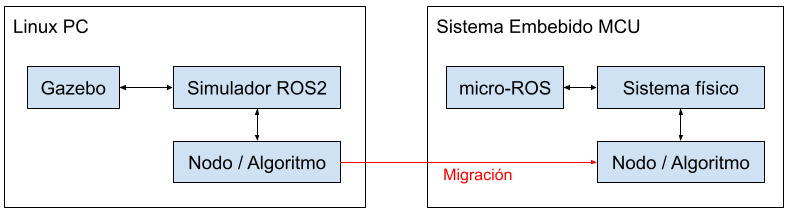
\includegraphics[width=.8\textwidth]{./Figuras/ros2-microros-migration.png}
\caption{Migración de algoritmos en entorno de simulación a sistema físico.}
\label{fig:ros2-to-microros}
\end{figure}

% El uso de micro-ROS permite continuar con el uso de todas las herramientas que facilita ROS 2, manteniendo el entorno de estudio del sistema, e inclusive posibilitando la realimentación del sistema físico hacia el entorno de simulación.

El entorno ROS es un framework de software libre y de código abierto diseñado para permitir el desarrollo de aplicaciones robóticas distribuidas. Este framework proporciona un conjunto de herramientas para la creación, gestión, depuración y análisis de sistemas robóticos.

La segunda versión de la herramienta, denominada ROS 2, fue desarrollada por la comunidad con el objetivo de mejorar la escalabilidad, la fiabilidad y la seguridad del software.
Una de sus principales características es que está diseñado para ser modular y extensible, lo que significa que los desarrolladores pueden elegir los componentes que necesitan para sus aplicaciones y utilizarlos de manera flexible. 
También se enfoca en proporcionar una abstracción de hardware más clara y permitir el uso de diferentes sistemas operativos y arquitecturas. 

La herramienta micro-ROS es una implementación de ROS 2 diseñada específicamente para sistemas embebidos y de tiempo real. A diferencia de ROS 2, que se ejecuta en sistemas operativos de propósito general, micro-ROS se ejecuta en sistemas operativos de tiempo real (como NuttX y FreeRTOS), lo que permite el desarrollo de sistemas robóticos en entornos de baja potencia y recursos limitados.

Como puede observarse en la figura \ref{fig:microROSarch}, micro-ROS proporciona una capa de abstracción que permite la comunicación entre los sistemas embebidos y los nodos de ROS 2 en otros sistemas.
Esto significa que los desarrolladores pueden crear sistemas robóticos distribuidos, que utilicen tanto sistemas embebidos como sistemas de propósito general y que todos ellos puedan comunicarse a través de la misma plataforma.

\begin{figure}[htpb]
\centering 
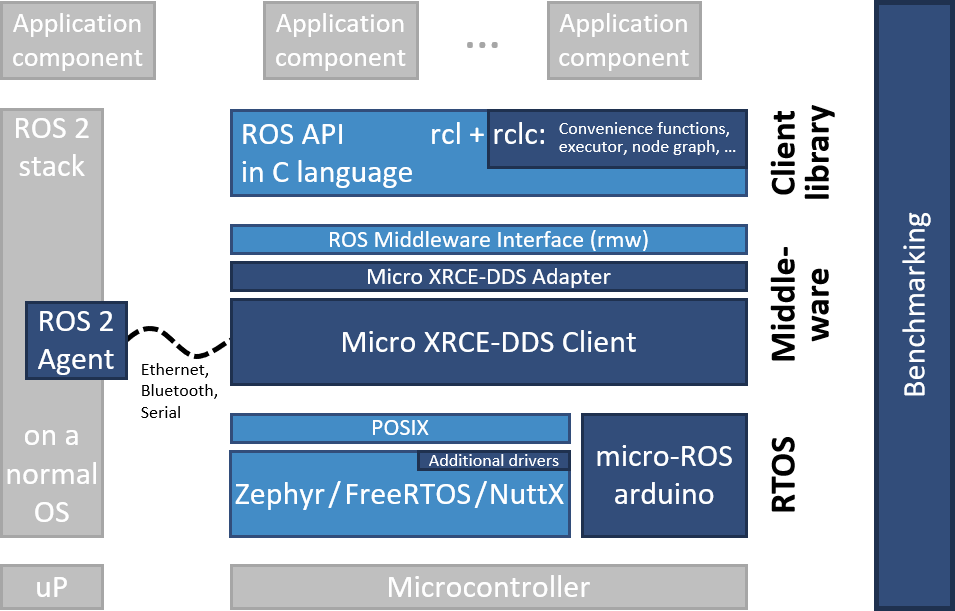
\includegraphics[width=.7\textwidth]{./Figuras/micro-ROS_architecture.png}
\caption{Arquitectura de micro-ROS.}
\label{fig:microROSarch}
\end{figure}

\section{2. Identificación y análisis de los interesados}
\label{sec:interesados}

\begin{table}[ht]
%\caption{Identificación de los interesados}
%\label{tab:interesados}
\begin{tabularx}{\linewidth}{@{}|l|X|X|l|@{}}
\hline
\rowcolor[HTML]{C0C0C0} 
Rol           & Nombre y Apellido & Organización 	& Puesto 	\\ \hline
% Auspiciante   &                   &              	&        	\\ \hline
Cliente       & \clientename      &\empclientename	&  Investigador      	\\ \hline
% Impulsor      &                   &              	&        	\\ \hline
Responsable   & \authorname       & FIUBA        	& Alumno 	\\ \hline
% Colaboradores &                   &              	&        	\\ \hline
Orientador    & \supname	      & \pertesupname 	& Director Trabajo final \\ \hline
Equipo        & Evangelina Castellano          &        Universidad Nacional de Córdoba    	&     Colaboradores   	\\ \hline
%Opositores    &                   &              	&        	\\ \hline
Usuario final & Grupos de investigación                  &   Fundación Fulgor           	&     -   	\\ \hline
\end{tabularx}
\end{table}

\begin{itemize}
	\item Cliente: el \clientename{} se encuentra haciendo su doctorado en la Fundación Fulgor y posee un gran conocimiento sobre los algoritmos utilizados para navegación autónoma a alto nivel. Es capaz de resolver dudas específicas sobre los requerimientos a cumplir con el algoritmo a implementar.
	\item Orientador: el \supname{} finalizó a finales de 2022 su doctorado en Mecatrónica, Robótica e Ingeniería de Automatización en Isae-Supaero, Toulouse, Francia. Actualmente se encuentra trabajando en Nimble One como investigador especialista en locomoción robótica. Se encuentra ubicado en Toulouse, Francia, y se mantendrán reuniones remotas cada dos semanas. La periodicidad de las reuiniones se ajustará segun lo demanden las actividades del proyecto y la disponibilidad del responsable y el orientador.
	\item Equipo: Evangelina Castellano se encuentra realizando su Práctica Profesional Supervisada (PPS) en la Fundación Fulgor. Al finalizar su PPS continuará en la institución para realizar su proyecto final de grado. Es necesario planificar teniendo en cuenta que la dedicación es simple, es decir, entre 4 y 5 horas diarias.
	\item Usuario final: no esta representado por una persona particular. Una vez finalizado el proyecto el prototipo quedará disponible en la Fundación Fulgor para su uso.
\end{itemize}

\section{3. Propósito del proyecto}
\label{sec:proposito}

El propósito de este proyecto es desarrollar el prototipo de una plataforma de hardware con las capacidades para poder implementar los algoritmos investigados de SLAM monocular y observar resultados.

La técnica de SLAM monocular es de interés por su aplicación en la navegación autónoma de vehículos, su bajo costo económico y simpleza del hardware involucrado en comparación a otras técnicas utilizadas en el área.

\section{4. Alcance del proyecto}
\label{sec:alcance}

El proyecto incluye el diseño del sistema embebido, el desarrollo de los drivers de los sensores asociados a las técnicas de SLAM monocular, la incorporación de la interfaz de micro-ROS en el proyecto, la aplicación de ROS 2 que permitirá interactuar con el sistema a alto nivel y la investigación e implementación de un algoritmo de SLAM monocular adecuado.

El proyecto no incluye el desarrollo de algoritmos de navegación autónoma asociados a la planificación y ejecución de trayectorias del vehículo, ni el modelado matemático de este. Tampoco incluye optimización de los algoritmos planteados con el uso de hardware dedicado como una FPGA, por ser una actividad que se realizará en una segunda etapa del proyecto.

Por lo tanto, el producto final esperado es un prototipo de un sistema embebido con los correspondientes sensores y herramientas necesarias funcionando en conjunto con técnicas de SLAM monocular, que un vehículo móvil pueda incorporar para dotarlo con capacidades de navegación autónoma.

\section{5. Supuestos del proyecto}
\label{sec:supuestos}

Para el desarrollo del presente proyecto se supone que:

\begin{itemize}
	\item La adquisición de materiales no tendrá demoras mayores a una semana, asumiendo que el mercado local posee los materiales requeridos para la fabricación del prototipo.
	\item No habrá cambios en el equipo de trabajo en el periodo de tiempo que comprende la planificación del proyecto.
	\item El responsable del proyecto puede dedicar una cantidad mínima de 25 horas semanales a las actividades del plan.
	\item El responsable del proyecto estará ausente durante dos semanas de Julio del año 2023, con fecha a definir.
	\item No habrá cambios en los objetivos principales del proyecto ni nuevos requerimientos funcionales de parte del cliente.
\end{itemize}

\section{6. Requerimientos}
\label{sec:requerimientos}

\begin{enumerate}
\item Requerimientos funcionales:
\begin{enumerate}
	\item El driver de la Unidad de Medición Inercial (IMU por sus siglas en inglés) debe ofrecer la información del giróscopo y acelerómetro de forma completa a la aplicación.
	\item El sistema debe utilizar algoritmos y técnicas de fusión sensorial para optimizar el uso de la información obtenida por la IMU.
	\item El driver de la IMU debe brindar todas las posibilidades de configuración necesarias para poder adaptar la escala y frecuencia de muestreo de los sensores a los requisitos de la aplicación.
	\item El driver de la cámara debe proveer la información correcta a la aplicación, dadas las capacidades del dispositivo.
	\item El driver de la IMU y de la cámara deben implementarse de forma modular para que puedan utilizarse independientemente del proyecto.
	\item El sistema embebido debe utilizar micro-ROS para interactuar e integrarse fácilmente con el entorno de desarrollo, monitoreo y evaluación de ROS 2.
	\item El sistema embebido debe hacer un uso adecuado de los mecanismos de comunicación de micro-ROS con ROS 2 para explotar todas las ventajas que ofrece el framework.
	\item El sistema debe estar diseñado de forma modular para favorecer su escalabilidad.
	\item El sistema debe ejecutar un algoritmo investigado previamente de SLAM monocular.
\end{enumerate}

\item Requerimientos de documentación:
\begin{enumerate}
	\item Todas aquellas funcionalidades cubiertas en el driver de la IMU deben estar completamente documentadas para que el módulo de software pueda utilizarse independientemente del proyecto.
	\item El proceso de incorporación y uso de las librerías de micro-ROS debe estar correctamente documentado para facilitar el desarrollo continuo del sistema.
	\item La investigación del estado del arte en el tópico de algoritmos de SLAM monocular debe estar debidamente documentada.
	\item El algoritmo seleccionado para implementar en el sistema debe estar documentado en forma detallada.
\end{enumerate}

\item Requerimientos de testing:
\begin{enumerate}
	\item Se deben aplicar herramientas y metodologías de testing en los drivers de los módulos para asegurar su funcionamiento y calidad.
\end{enumerate}

\item Requerimientos de la interfaz:
\begin{enumerate}
	\item Las herramientas desarrolladas en el entorno de ROS 2 deben también cumplir el propósito de interfaz gráfica y permitir la visualización de la información obtenida a través de los sensores.
	\item El sistema desarrollado con ROS 2 debe ofrecer herramientas que permitan operar y reconfigurar el sistema.
	\item El sistema desarrollado con ROS 2 debe ofrecer herramientas que permitan evaluar el desempeño del algoritmo implementado, como puede ser el ajuste de parámetros del sistema \textit{on-the-fly}, la visualización del mapa del entorno y la ubicación espacial de la plataforma en él y otras herramientas que se consideren necesarias.
\end{enumerate}
\end{enumerate}

\section{7. Historias de usuarios (\textit{Product backlog})}
\label{sec:backlog}

Se identifican los siguientes roles/usuarios:
\begin{enumerate}
	\item Investigador en el área de Ciencias de la Computación, en su rol de estudiante de máster o PhD desea realizar avances en los algoritmos de navegación autónoma. No necesariamente tiene conocimientos de electrónica y sistemas embebidos, su foco es el desarrollo de alto nivel.
	\item Investigador en el área de la electrónica, sistemas embebidos y/o firmware, en su rol de estudiante de máster o PhD desea realizar avances en el desarrollo de dispositivos de navegación autónoma mediante la optimización o mejora del hardware y el firmware asociado.
	\item Usuario perteneciente a la comunidad de código abierto/libre, en su rol desea implementar el proyecto con sus propios materiales, aplicarlo en un caso de uso específico y colaborar con posibles mejoras. Puede o no poseer conocimiento técnico.
\end{enumerate}

La ponderación de cada historia de usuario se obtiene de una evaluación sobre tres ejes: tiempo, dificultad e incertidumbre. Sobre cada eje se asigna un valor en una escala entre 0 y 5, luego este valor se penaliza según la relevancia asignada a cada aspecto: tiempo 0.4, dificultad 0.2 e incertidumbre 0.4. Para obtener el puntaje final de la historia se divide el resultado parcial por 5 y se multiplica por 100.

\textbf{Historia 1 de usuario 1:} como investigador en el área de Ciencias de la Computación quiero poder utilizar los sensores de SLAM monocular como si fueran una caja negra, quiero que sea sencillo aprender a utilizarlo e incorporarlo en mi flujo de trabajo para bajar de forma sencilla al dispositivo los algoritmos implementados a alto nivel en la simulación.

\begin{itemize}
	\item Tiempo: 4
	\item Dificultad: 3
	\item Incertidumbre: 2
	\item Puntaje: 60 
\end{itemize}

\textbf{Historia 2 de usuario 1:} como investigador en el área de Ciencias de la Computación quiero poder visualizar la información obtenida por los sensores y utilizarla como entrada a simulaciones virtuales.

\begin{itemize}
	\item Tiempo: 3
	\item Dificultad: 2
	\item Incertidumbre: 1
	\item Puntaje: 40
\end{itemize}

\textbf{Historia 1 de usuario 2:} como investigador en el área de la electrónica quiero poder entender rápido cómo esta conformado el sistema y que sea lo suficientemente modular como para modificar, mejorar y/o intercambiar algún componente funcional y que el sistema siga operando sin dificultades.

\begin{itemize}
	\item Tiempo: 4
	\item Dificultad: 3
	\item Incertidumbre: 2
	\item Puntaje: 60
\end{itemize}

\textbf{Historia 2 de usuario 2:} como investigador en el área de la electrónica quiero poder reutilizar los componentes que conforman el sistema de forma independiente en un proyecto diferente.

\begin{itemize}
	\item Tiempo: 3
	\item Dificultad: 3
	\item Incertidumbre: 2
	\item Puntaje: 52
\end{itemize}

\textbf{Historia 1 de usuario 3:} como parte de la comunidad de código abierto/libre quiero que los materiales utilizados en el prototipo sean accesibles y que el proyecto tenga la documentación completa de las distintas etapas para poner en marcha el sistema.

\begin{itemize}
	\item Tiempo: 5
	\item Dificultad: 1
	\item Incertidumbre: 3
	\item Puntaje: 68
\end{itemize}

\textbf{Historia 2 de usuario 3:} como parte de la comunidad de código abierto/libre quiero que el proyecto posea un mecanismo para poder contribuir en cualquiera de sus aspectos dado mi conocimiento específico.

\begin{itemize}
	\item Tiempo: 4
	\item Dificultad: 2
	\item Incertidumbre: 3
	\item Puntaje: 64
\end{itemize}

\section{8. Entregables principales del proyecto}
\label{sec:entregables}

Los entregables del proyecto son:
\begin{itemize}
	\item Plataforma de hardware que conforma el prototipo funcional
	\item Documentación del hardware e interconexión de los módulos componentes
	\item Código fuente del driver de la IMU
	\item Documentación del driver de la IMU
	\item Código fuente del driver de la cámara
	\item Documentación del driver de la cámara
	\item Código fuente del firmware con el algoritmo de SLAM monocular y micro-ROS
	\item Código fuente del agente de ROS 2 utilizado
	\item Documentación y manual para configuración y uso del entorno de ROS 2
	\item Documentación del estado del arte de SLAM y del algoritmo seleccionado
	\item Manual de uso del hardware
	\item Informe final
\end{itemize}

\section{9. Desglose del trabajo en tareas}
\label{sec:wbs}

\begin{enumerate}
	\item Planificación del proyecto (70 h)
	\begin{enumerate}
		\item Identificación y contacto con los interesados (7 h)
		\item Definición del propósito y alcance del proyecto (10 h)
		\item Definición de los requerimientos y entregables (20 h)
		\item Desglose del trabajo en tareas y obtención del diagrama de Gantt (20 h)
		\item Análisis de riesgos, gestión de calidad y definición de procesos de cierre (13 h)
	\end{enumerate}
	\item Setup del entorno de trabajo para desarrollo del software necesario (5 h)
	\item Implementación de micro-ROS en el sistema embebido (18 h)
	\begin{enumerate}
		\item Introducción a micro-ROS (4 h)
		\item Incorporación de micro-ROS en el microcontrolador (8 h)
		\item Setup de agente de ROS 2 y comunicación con sistema embebido (2 h)
		\item Documentación del proceso (4 h)
	\end{enumerate}
	\item Desarrollo de driver para la IMU (40 h)
	\begin{enumerate}
		\item Selección y adquisición de la IMU a utilizar (2 h)
		\item Implementación de driver en lenguaje C para el sistema embebido (30 h)
		\item Documentación del driver (8 h)
	\end{enumerate}
	\item Integración de la IMU en el sistema (60 h)
	\begin{enumerate}
		\item Integración de driver de la IMU con el sistema con micro-ROS (4 h)
		\item Repaso (e investigación) de técnicas de fusión sensorial (8 h)
		\item Implementación de algoritmos de fusión sensorial (30 h)
		\item Visualización de la información obtenida con la IMU mediante las herramientas de ROS 2 (10 h)
		\item Evaluación parcial y documentación de resultados (milestone) (8 h)
	\end{enumerate}
	\item Desarrollo de driver para la cámara (53 h)
	\begin{enumerate}
		\item Selección y adquisición de cámara a utilizar (3 h)
		\item Implementación de driver en lenguaje C para el sistema embebido (40 h)
		\item Documentación del driver (10 h)
	\end{enumerate}
	\item Integración de la cámara en el sistema (26 h)
	\begin{enumerate}
		\item Integración del driver de la cámara con el sistema con micro-ROS (6 h)
		\item Visualización de la información obtenida con la cámara mediante las herramientas de ROS 2 (12 h)
		\item Evaluación parcial y documentación de resultados (milestone) (8 h)
	\end{enumerate}
	\item Implementación de algoritmo de SLAM monocular (305 h)
	\begin{enumerate}
		\item Introducción a la navegación inercial y SLAM monocular, investigación de estado del arte (15 h)
		\item Investigación de algoritmos de SLAM monocular y selección de uno de ellos (30 h)
		\item Implementación del algoritmo seleccionado en un entorno de simulación (40 h)
		\item Optimización del algoritmo implementado en el entorno de simulación (40 h)
		\item Evaluación integral de los componentes del sistema (20 h)
		\item Implementación del algoritmo seleccionado sobre la plataforma desarrollada (40 h)
		\item Optimización del algoritmo implementado sobre la plataforma desarrolada (40 h)
		\item Evaluación final de resultados (milestone) (40 h)
		\item Documentación técnica del algoritmo seleccionado y resumen del estado del arte (40 h)
	\end{enumerate}
	\item Proceso de cierre (91 h)
	\begin{enumerate}
		\item Análisis de cumplimiento de objetivos y requerimientos con el director (2 h)
		\item Análisis de cumplimiento del plan original (diagrama de Gantt) (2 h)
		\item Análisis de cumplimiento de objetivos y requerimientos con el cliente (2 h)
		\item Elaboración de memoria técnica (40 h)
		\item Corrección de memoria técnica (20 h)
		\item Preparación de defensa pública (20 h)
		\item Defensa pública (2 h)
		\item Reunión de cierre con el director (1 h)
		\item Reunión de cierre con el cliente y el equipo de trabajo (2 h)
	\end{enumerate}
\end{enumerate}

Cantidad total de horas: 668 h

\section{10. Diagrama de Activity On Node}
\label{sec:AoN}

Las tareas expuestas en el diagrama de \textit{Activity On Node}, figura \ref{fig:AoN}, se encuentran explicitadas en la siguiente tabla, con su código, duración y tareas predecesoras.

% Please add the following required packages to your document preamble:
% \usepackage{booktabs}
\begin{table}[htpb]
\centering
%\caption{WBS: Desglose del trabajo en tareas.}
\label{tab:wbs}
\begin{tabular}{@{}llll@{}}
\toprule
\textbf{Código} & \textbf{Predecesora} & \textbf{Descripción}                               & \textbf{Duración} \\ \midrule
1               &                      & Planificación del proyecto                         & 70 h               \\
1.1             &                      & Identificación y contacto con los interesados       & 7 h                \\
1.2             & 1.1                  & Definición del propósito y alcance del proyecto    & 10 h               \\
1.3             & 1.2                  & Definición de los requerimientos y entregables     & 20 h               \\
1.4             & 1.3                  & Desglose del trabajo en tareas                     & 20 h               \\
1.5             & 1.4                  & Análisis de riesgos y gestión de calidad           & 13 h               \\
2               & 1                    & Setup del entorno de trabajo                       & 5 h                \\
3               &                      & Implementación de micro-ROS                        & 18 h               \\
3.1             & 1                    & Introducción a micro-ROS                           & 4 h                \\
3.2             & 2, 3.1               & Incorporación de micro-ROS en el sistema           & 8 h                \\
3.3             & 3.2                  & Setup del agente de ROS 2                          & 2 h                \\
3.4             & 3.3                  & Documentación del proceso                          & 4 h                \\
4               &                      & Desarrollo de driver para la IMU                   & 40 h               \\
4.1             & 1                    & Selección y adquisición de la IMU a utilizar       & 2 h                \\
4.2             & 2, 4.1               & Implementación de driver para el sistema embebido  & 30 h               \\
4.3             & 4.2                  & Documentación del driver                           & 8 h                \\
5               &                      & Integración de la IMU en el sistema                & 60 h               \\
5.1             & 3.3, 4.2             & Integración del driver de la IMU con micro-ROS     & 4 h                \\
5.2             & 1                    & Repaso de técnicas de fusión sensorial             & 8 h                \\
5.3             & 4.2, 5.2             & Implementación de algoritmos de fusión sensorial   & 30 h               \\
5.4             & 5.1                  & Visualización de la información mediante ROS 2     & 10 h               \\
5.5             & 5.3, 5.4             & Evaluación parcial de resultados y documentación   & 8 h                \\
6               &                      & Desarrollo de driver para la cámara                & 53 h               \\
6.1             & 1                    & Selección y adquisición de la cámara a utilizar    & 3 h                \\
6.2             & 2, 6.1               & Implementación de driver para el sistema embebido  & 40 h               \\
6.3             & 6.2                  & Documentación del driver                           & 10 h               \\
7               &                      & Integración de la cámara en el sistema             & 26 h               \\
7.1             & 3.3, 6.2             & Integración del driver de la cámara con micro-ROS  & 6 h                \\
7.2             & 7.1                  & Visualización de la información mediante ROS 2     & 12 h               \\
7.3             & 7.2                  & Evaluación parcial de resultados y documentación   & 8 h                \\
8               &                      & Implementación de algoritmo de SLAM monocular      & 305 h              \\
8.1             & 1                    & Investigación del estado del arte de SLAM          & 15 h               \\
8.2             & 8.1                  & Investigación y selección de algoritmos de SLAM    & 30 h               \\
8.3             & 2, 8.2               & Implementación del algoritmo en simulación         & 40 h               \\
8.4             & 8.3                  & Optimización del algoritmo en simulación           & 40 h               \\
8.5             & 5.5, 7.3             & Evaluación integral de los componentes del sistema & 20 h               \\
8.6             & 8.4, 8.5             & Implementación del algoritmo en el sistema embebido  & 40 h               \\
8.7             & 8.6                  & Optimización del algoritmo en el sistema embebido  & 40 h               \\
8.8             & 8.7                  & Evaluación final de resultados                     & 40 h               \\
8.9             & 8.8                  & Documentación técnica del algoritmo                & 50 h               \\
9               &                      & Proceso de cierre                                  & 91 h               \\ 
9.1             & 8.9                  & Análisis de cumplimiento de objetivos con director & 2 h                \\ 
9.2             & 9.1                  & Análisis de cumplimiento del plan original         & 2 h                \\ 
9.3             & 9.2                  & Análisis de cumplimiento de objetivos con cliente  & 2 h                \\ 
9.4             & 9.3                  & Elaboración de memoria técnica                     & 40 h               \\ 
9.5             & 9.4                  & Corrección de memoria técnica                      & 20 h               \\
9.6             & 9.5                  & Preparación de defensa pública                     & 20 h               \\
9.7             & 9.6                  & Defensa pública                                    & 2 h                \\
9.8             & 9.7                  & Reunión de cierre con director                     & 1 h                \\
9.9             & 9.8                  & Reunión de cierre con cliente y equipo de trabajo  & 2 h                \\ \bottomrule
\end{tabular}
\end{table}

% \begin{consigna}{red}
% Armar el AoN a partir del WBS definido en la etapa anterior. 

%La figura \ref{fig:AoN} fue elaborada con el paquete latex tikz y pueden consultar la siguiente referencia \textit{online}:

%\url{https://www.overleaf.com/learn/latex/LaTeX_Graphics_using_TikZ:_A_Tutorial_for_Beginners_(Part_3)\%E2\%80\%94Creating_Flowcharts}

% \end{consigna}

\begin{landscape}
\begin{figure}[htpb]
\centering 
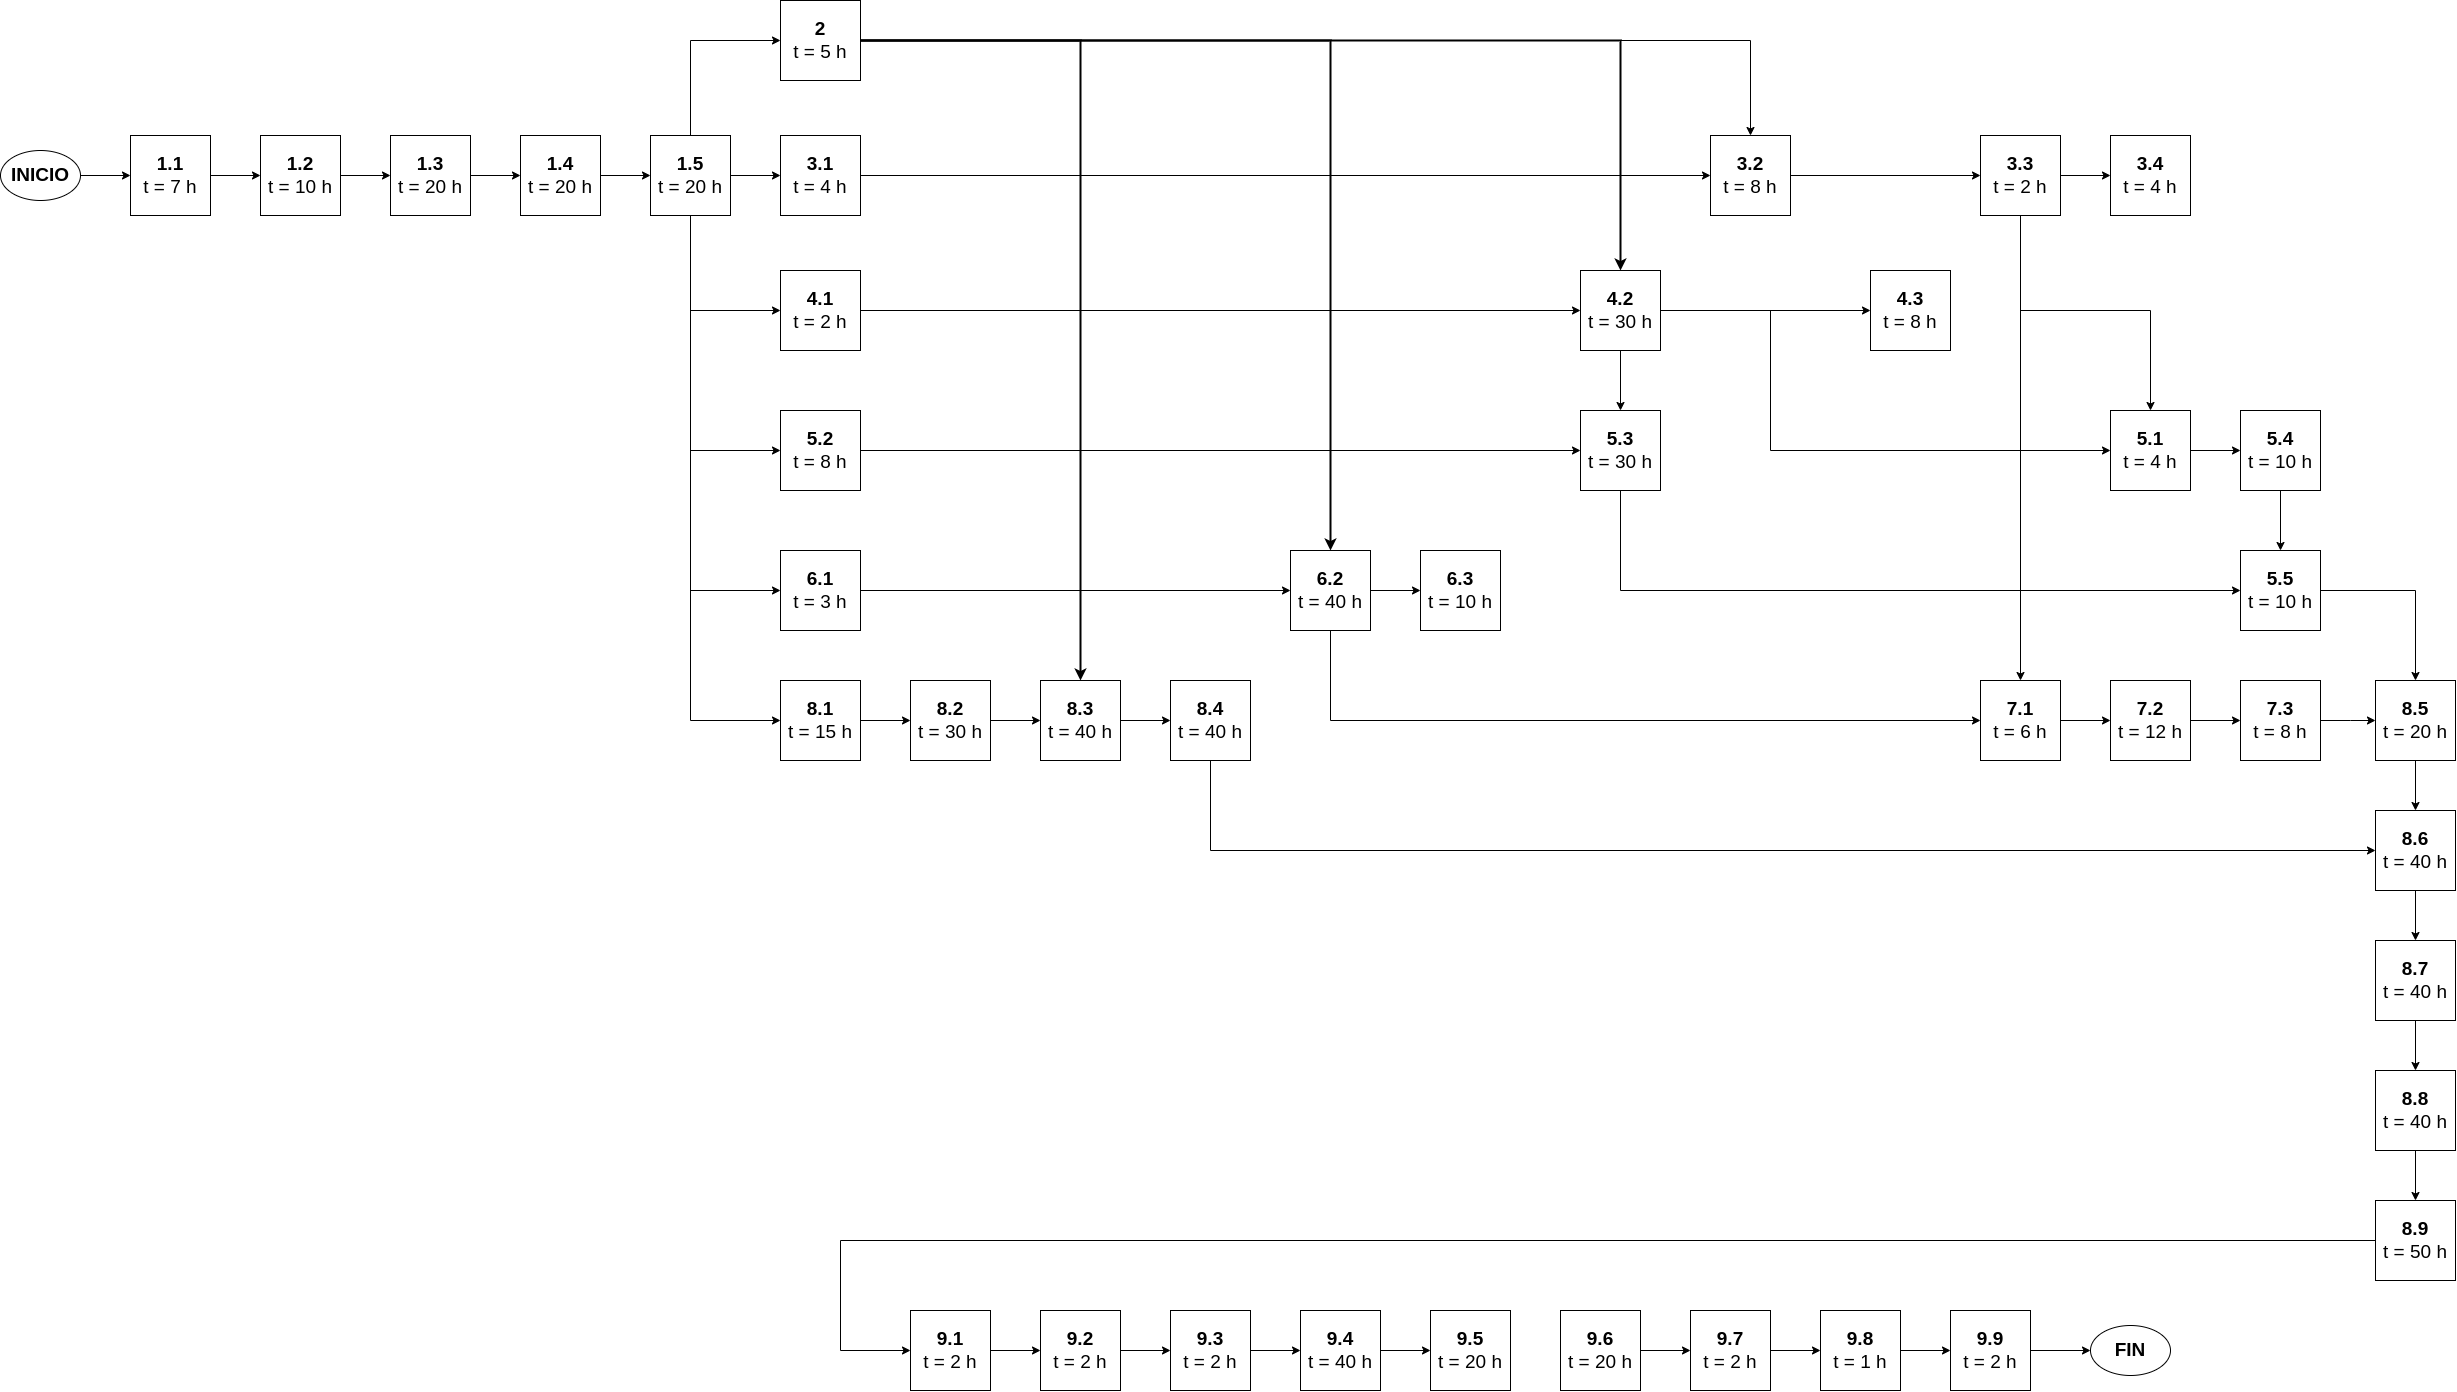
\includegraphics[width=1.5\textwidth]{./Figuras/MonoSLAM-AoN.png}
\caption{Diagrama de \textit{Activity on Node}.}
\label{fig:AoN}
\end{figure}
\end{landscape}

% Indicar claramente en qué unidades están expresados los tiempos.
% De ser necesario indicar los caminos semicríticos y analizar sus tiempos mediante un cuadro.
% Es recomendable usar colores y un cuadro indicativo describiendo qué representa cada color, como se muestra en el siguiente ejemplo:

% \begin{consigna}{red}

% Existen muchos programas y recursos \textit{online} para hacer diagramas de Gantt, entre los cuales destacamos:

% \begin{itemize}
% \item Planner
% \item GanttProject
% \item Trello + \textit{plugins}. En el siguiente link hay un tutorial oficial: \\ \url{https://blog.trello.com/es/diagrama-de-gantt-de-un-proyecto}
% \item Creately, herramienta online colaborativa. \\\url{https://creately.com/diagram/example/ieb3p3ml/LaTeX}
% \item Se puede hacer en latex con el paquete \textit{pgfgantt}\\ \url{http://ctan.dcc.uchile.cl/graphics/pgf/contrib/pgfgantt/pgfgantt.pdf}
% \end{itemize}

% Pegar acá una captura de pantalla del diagrama de Gantt, cuidando que la letra sea suficientemente grande como para ser legible. 
% Si el diagrama queda demasiado ancho, se puede pegar primero la ``tabla'' del Gantt y luego pegar la parte del diagrama de barras del diagrama de Gantt.

% Configurar el software para que en la parte de la tabla muestre los códigos del EDT (WBS).\\
% Configurar el software para que al lado de cada barra muestre el nombre de cada tarea.\\
% Revisar que la fecha de finalización coincida con lo indicado en el Acta Constitutiva.

% En la figura \ref{fig:gantt}, se muestra un ejemplo de diagrama de Gantt realizado con el paquete de \textit{pgfgantt}. En la plantilla pueden ver el código que lo genera y usarlo de base para construir el propio.

% \begin{figure}[htbp]
% \begin{center}
% \begin{ganttchart}{1}{12}
%   \gantttitle{2020}{12} \\
%   \gantttitlelist{1,...,12}{1} \\
%   \ganttgroup{Group 1}{1}{7} \\
%   \ganttbar{Task 1}{1}{2} \\
%   \ganttlinkedbar{Task 2}{3}{7} \ganttnewline
%   \ganttmilestone{Milestone o hito}{7} \ganttnewline
%   \ganttbar{Final Task}{8}{12}
%   \ganttlink{elem2}{elem3}
%   \ganttlink{elem3}{elem4}
% \end{ganttchart}
% \end{center}
% \caption{Diagrama de Gantt de ejemplo}
% \label{fig:gantt}
% \end{figure}


% \begin{landscape}
% \begin{figure}[htpb]
% \centering 
% 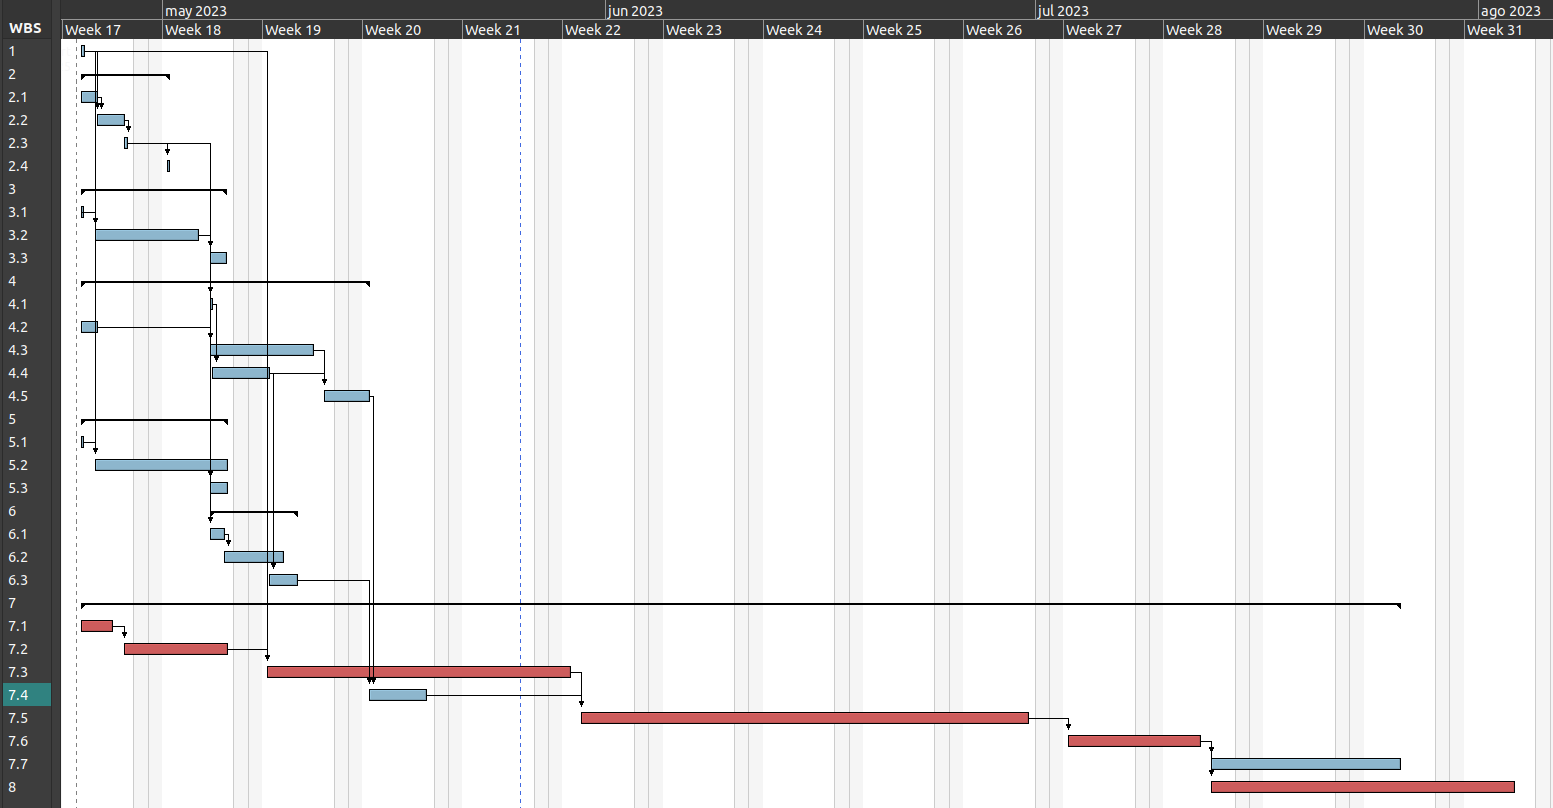
\includegraphics[height=.85\textheight]{./Figuras/Gantt_v1.png}
% \caption{Ejemplo de diagrama de Gantt rotado}
% \label{fig:diagGantt}
% \end{figure}
% \end{landscape}

% \end{consigna}

\begin{landscape}
\section{11. Diagrama de Gantt}
\label{sec:gantt}
\begin{figure}[htpb]
\centering 
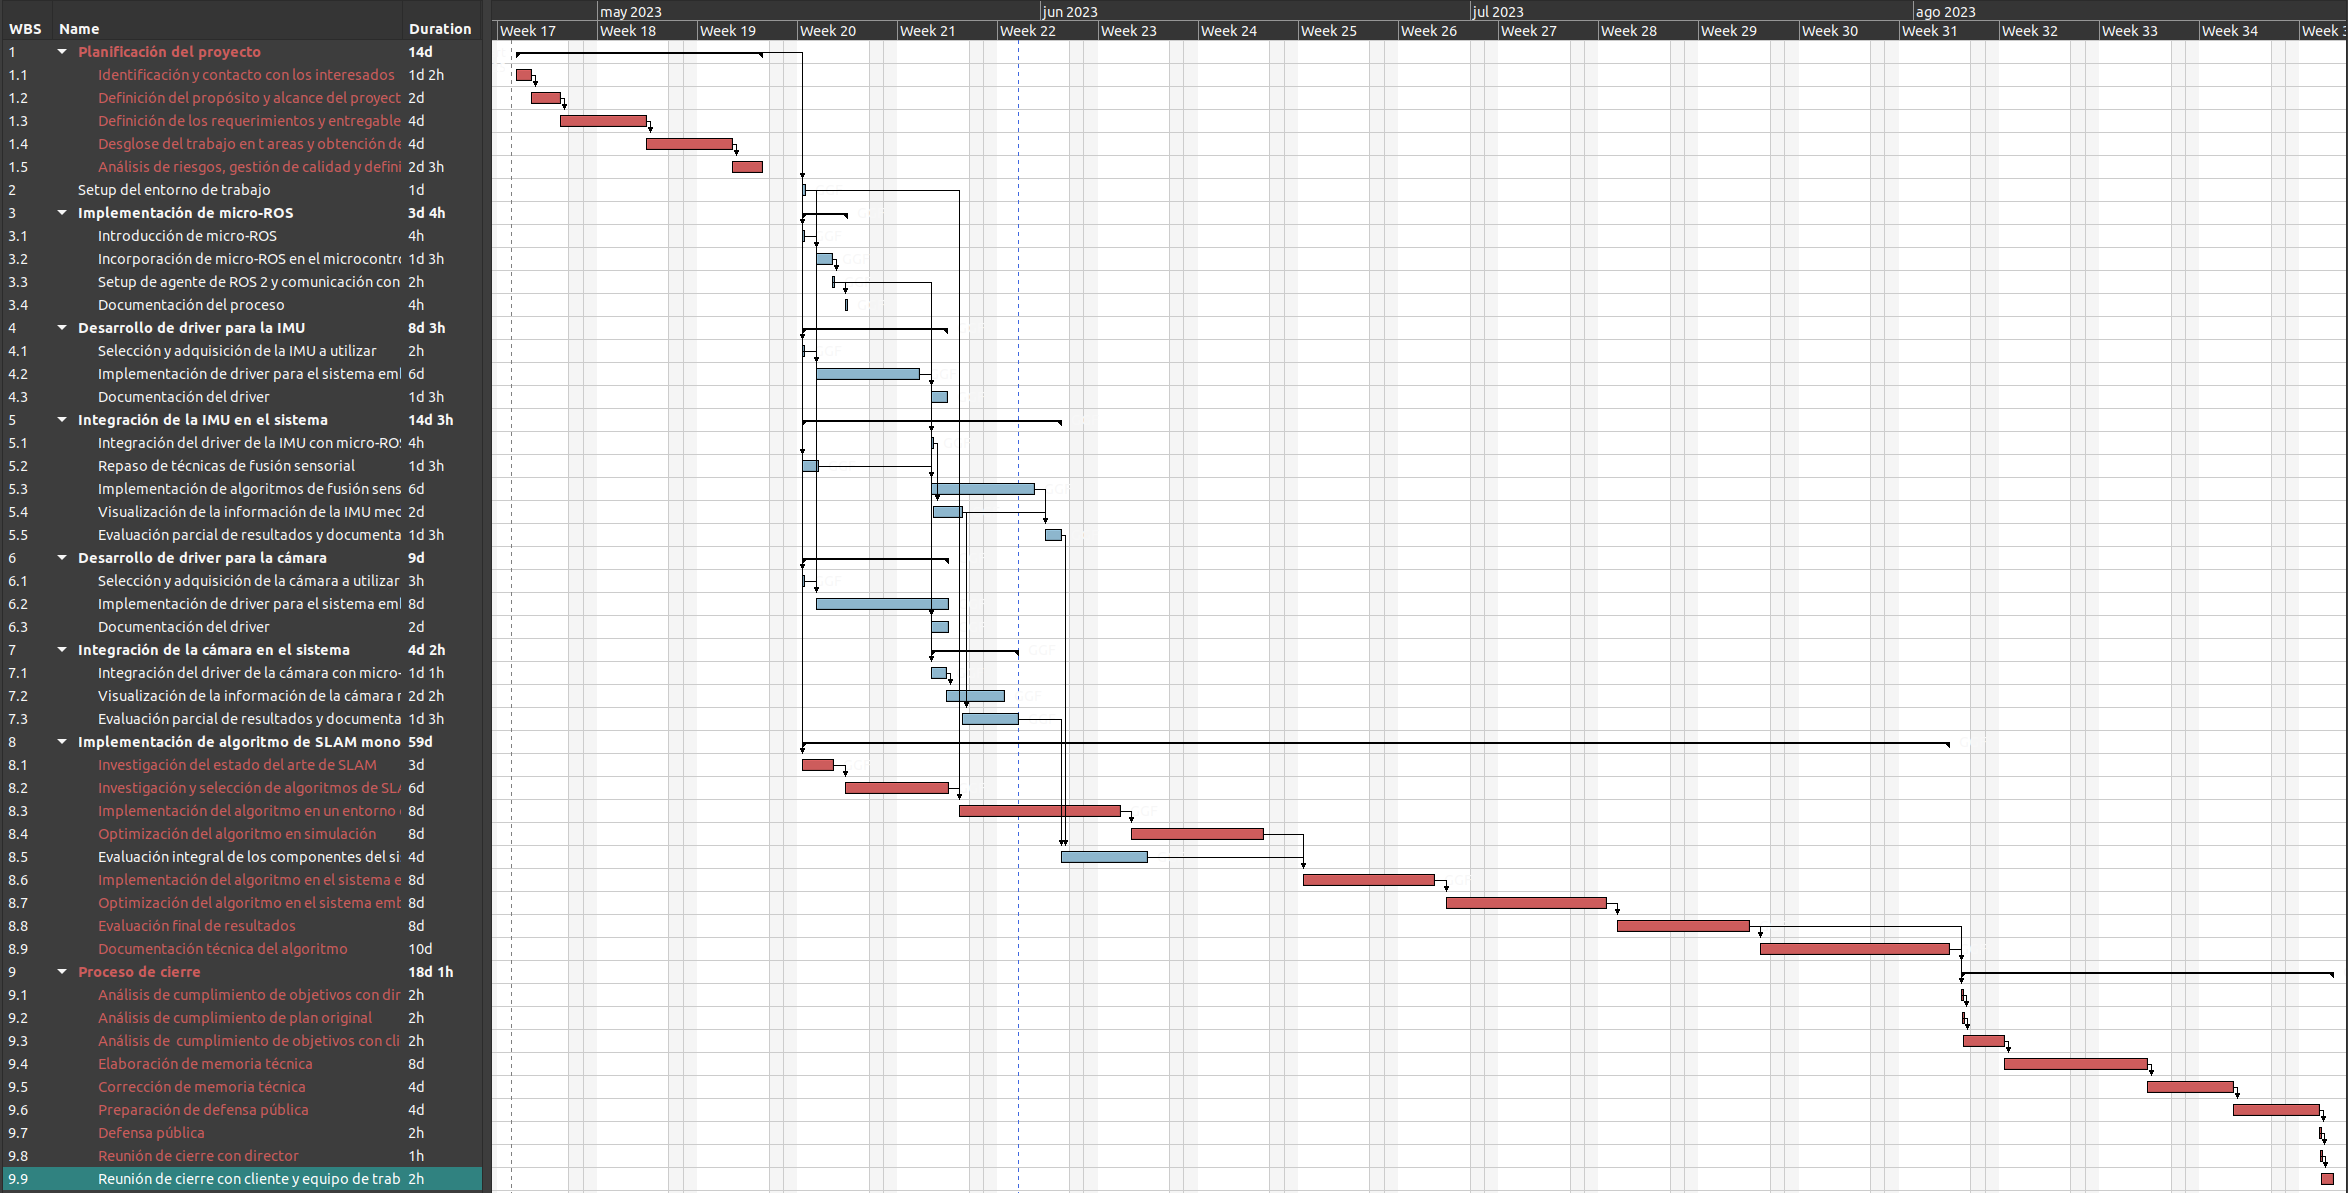
\includegraphics[height=.77\textheight]{./Figuras/Gantt_v2.png}
%\caption{Diagrama de Gantt del proyecto.}
\label{fig:diagGantt}
\end{figure}
\end{landscape}


\section{12. Presupuesto detallado del proyecto}
\label{sec:presupuesto}

\begin{table}[htpb]
\centering
\begin{tabularx}{\linewidth}{@{}|X|c|r|r|@{}}
\hline
\rowcolor[HTML]{C0C0C0} 
\multicolumn{4}{|c|}{\cellcolor[HTML]{C0C0C0}COSTOS DIRECTOS} \\ \hline
\rowcolor[HTML]{C0C0C0} 
Descripción &
  \multicolumn{1}{c|}{\cellcolor[HTML]{C0C0C0}Cantidad} &
  \multicolumn{1}{c|}{\cellcolor[HTML]{C0C0C0}Valor unitario} &
  \multicolumn{1}{c|}{\cellcolor[HTML]{C0C0C0}Valor total} \\ \hline
Placa de desarrollo STM32 Nucleo &
  \multicolumn{1}{c|}{1} &
  \multicolumn{1}{c|}{30000 ARS} &
  \multicolumn{1}{c|}{30000 ARS} \\ \hline
Cámara &
  \multicolumn{1}{c|}{1} &
  \multicolumn{1}{c|}{5000 ARS} &
  \multicolumn{1}{c|}{5000 ARS} \\ \hline
\multicolumn{1}{|l|}{Unidad de medición inercial} &
  \multicolumn{1}{c|}{1} &
  \multicolumn{1}{c|}{5000 ARS} &
  \multicolumn{1}{c|}{5000 ARS} \\ \hline
\multicolumn{1}{|l|}{Componentes de electrónica varios} &
  \multicolumn{1}{c|}{1} &
  \multicolumn{1}{c|}{3000 ARS} &
  \multicolumn{1}{c|}{3000 ARS} \\ \hline
\multicolumn{1}{|l|}{Hora de ingeniería} &
  \multicolumn{1}{c|}{668} &
  \multicolumn{1}{c|}{2500 ARS} &
  \multicolumn{1}{c|}{1670000 ARS} \\ \hline
\multicolumn{3}{|c|}{SUBTOTAL} &
  \multicolumn{1}{c|}{1713000 ARS} \\ \hline
\rowcolor[HTML]{C0C0C0} 
\multicolumn{4}{|c|}{\cellcolor[HTML]{C0C0C0}COSTOS INDIRECTOS} \\ \hline
\rowcolor[HTML]{C0C0C0} 
Descripción &
  \multicolumn{1}{c|}{\cellcolor[HTML]{C0C0C0}Cantidad} &
  \multicolumn{1}{c|}{\cellcolor[HTML]{C0C0C0}Valor unitario} &
  \multicolumn{1}{c|}{\cellcolor[HTML]{C0C0C0}Valor total} \\ \hline
\multicolumn{1}{|l|}{Transporte} &
  \multicolumn{1}{c|}{10} &
  \multicolumn{1}{c|}{100 ARS} &
  \multicolumn{1}{c|}{1000 ARS} \\ \hline
\multicolumn{1}{|l|}{Energía eléctrica} &
  \multicolumn{1}{c|}{1} &
  \multicolumn{1}{c|}{2000 ARS} &
  \multicolumn{1}{c|}{2000 ARS} \\ \hline
\multicolumn{1}{|l|}{5\% de costos directos} &
  \multicolumn{1}{c|}{1} &
  \multicolumn{1}{c|}{85650 ARS} &
  \multicolumn{1}{c|}{85650 ARS} \\ \hline
\multicolumn{3}{|c|}{SUBTOTAL} &
  \multicolumn{1}{c|}{88650 ARS} \\ \hline
\rowcolor[HTML]{C0C0C0}
\multicolumn{3}{|c|}{TOTAL} & 1801650 ARS
   \\ \hline
\end{tabularx}%
\end{table}


\section{13. Gestión de riesgos}
\label{sec:riesgos}

% \begin{consigna}{red}
% a) Identificación de los riesgos (al menos cinco) y estimación de sus consecuencias:
 
% Riesgo 1: detallar el riesgo (riesgo es algo que si ocurre altera los planes previstos de forma negativa)
% \begin{itemize}
% 	\item Severidad (S): mientras más severo, más alto es el número (usar números del 1 al 10).\\
% 	Justificar el motivo por el cual se asigna determinado número de severidad (S).
% 	\item Probabilidad de ocurrencia (O): mientras más probable, más alto es el número (usar del 1 al 10).\\
% 	Justificar el motivo por el cual se asigna determinado número de (O). 
% \end{itemize}   

% Riesgo 2:
% \begin{itemize}
% 	\item Severidad (S): 
% 	\item Ocurrencia (O):
% \end{itemize}

% Riesgo 3:
% \begin{itemize}
% 	\item Severidad (S): 
% 	\item Ocurrencia (O):
% \end{itemize}


% b) Tabla de gestión de riesgos:      (El RPN se calcula como RPN=SxO)

% \begin{table}[htpb]
% \centering
% \begin{tabularx}{\linewidth}{@{}|X|c|c|c|c|c|c|@{}}
% \hline
% \rowcolor[HTML]{C0C0C0} 
% Riesgo & S & O & RPN & S* & O* & RPN* \\ \hline
%        &   &   &     &    &    &      \\ \hline
%        &   &   &     &    &    &      \\ \hline
%        &   &   &     &    &    &      \\ \hline
%        &   &   &     &    &    &      \\ \hline
%        &   &   &     &    &    &      \\ \hline
% \end{tabularx}%
% \end{table}

% Criterio adoptado: 
% Se tomarán medidas de mitigación en los riesgos cuyos números de RPN sean mayores a...

% Nota: los valores marcados con (*) en la tabla corresponden luego de haber aplicado la mitigación.

% c) Plan de mitigación de los riesgos que originalmente excedían el RPN máximo establecido:
 
% Riesgo 1: plan de mitigación (si por el RPN fuera necesario elaborar un plan de mitigación).
%   Nueva asignación de S y O, con su respectiva justificación:
%   - Severidad (S): mientras más severo, más alto es el número (usar números del 1 al 10).
%           Justificar el motivo por el cual se asigna determinado número de severidad (S).
%   - Probabilidad de ocurrencia (O): mientras más probable, más alto es el número (usar del 1 al 10).
%           Justificar el motivo por el cual se asigna determinado número de (O).

% Riesgo 2: plan de mitigación (si por el RPN fuera necesario elaborar un plan de mitigación).
 
% Riesgo 3: plan de mitigación (si por el RPN fuera necesario elaborar un plan de mitigación).

% \end{consigna}

a) Identificación de los riesgos y estimación de sus consecuencias:

Riesgo 1: la IMU o la cámara seleccionadas y adquiridas para el prototipo no tienen buen desempeño en la aplicación del proyecto.
\begin{itemize}
	\item Severidad (S): 6, porque impacta en la calidad del resultado final del prototipo, pero no impide la obtención de una primera versión de este. 
	\item Probabilidad de ocurrencia (O): 5, porque es un riesgo contemplado al tener un presupuesto acotado para la adquisición de materiales. Dadas las limitaciones del primer prototipo, se desarrollará una segunda versión con mejoras en estos aspectos, contemplando la adquisición de sensores en el extranjero, de ser necesario.
\end{itemize}

Riesgo 2: hay cambios o imprevistos (ej., licencias) en el equipo de trabajo.
\begin{itemize}
	\item Severidad (S): 8, porque el grupo de trabajo es reducido y por lo tanto poco flexible a limitaciones adicionales en los recursos humanos disponibles.
	\item Probabilidad de ocurrencia (O): 6, porque Evangelina Castellano, colaboradora en el proyecto, puede inclinarse por otra temática para su proyecto final de grado una vez finalizada su PPS.
\end{itemize}

Riesgo 3: el responsable del proyecto puede dedicar menos de 25 horas semanales a las actividades del plan.
\begin{itemize}
	\item Severidad (S): 9, porque hay un único responsable y el equipo de trabajo es reducido.
	\item Probabilidad de ocurrencia (O): 3, porque solo ocurriría ante alguna situación personal o laboral particular.
\end{itemize}

Riesgo 4: hay cambios en los requerimientos funcionales del proyecto.
\begin{itemize}
	\item Severidad (S): 7, porque dependerá mucho de las características del requerimiento a añadir y de la instancia en la que se encuentra el proyecto.
	\item Probabilidad de ocurrencia (O): 6, porque pueden presentarse nuevas ideas que valga la pena explorar, tanto de parte del responsable como del cliente.
\end{itemize}

Riesgo 5: las limitaciones en el hardware impiden un buen desempeño del algoritmo investigado.
\begin{itemize}
	\item Severidad (S): 8, porque es un riesgo que, de presentarse, será en una instancia avanzada del proyecto.
	\item Probabilidad de ocurrencia (O): 6, porque es conocida la cantidad de recursos demandada por los algoritmos de SLAM.
\end{itemize}

b) Tabla de gestión de riesgos:

Criterio adoptado: se tomarán medidas de mitigación en los riesgos cuyos números de RPN sean igual o mayores a 40.
\begin{table}[htpb]
\centering
\begin{tabularx}{\linewidth}{@{}|X|c|c|c|c|c|c|@{}}
\hline
\rowcolor[HTML]{C0C0C0} 
Riesgo 													& S & O & RPN & S* & O* & RPN*  \\ \hline
1. Los sensores seleccionados no tienen buen desempeño. & 6 & 5 & 30  &   &     &  		\\ \hline
2. Cambios imprevistos en el equipo de trabajo       	& 8 & 6 & 48  & 6 & 6   & 36  	\\ \hline
3. Disponibilidad del responsable menor a la estimada.  & 9 & 3 & 27  &   &     &   	\\ \hline
4. Cambios en los requerimientos del proyecto.     		& 7 & 6 & 42 & 4  & 4   & 16  	\\ \hline
5. Limitación en el hardware impide buen desempeño     	& 8 & 6 & 48 & 7  & 4   & 28  	\\ \hline
\end{tabularx}%
\end{table}

c) Plan de mitigación de los riesgos que exceden el RPN máximo establecido:

Riesgo 2: se mantendrán reuniones mensuales con Evangelina Castellano y el \clientename{} para estar al tanto de su interés en el tema, el posible surgimiento de nuevas líneas de investigación más prioritarias o cualquier otra variable que pueda afectar al equipo de trabajo.
\begin{itemize}
	\item Severidad (S): 6, porque todavía existe la posibilidad de que haya cambios en el equipo de trabajo. Lo único que cambia es que se puede anticipar el cambio y adaptarse mediante la búsqueda de otro posible colaborador o realizando los ajustes necesarios en el plan de trabajo.
	\item Probabilidad de ocurrencia (O): 6, ya que el plan de mitigación no afecta esta variable.
\end{itemize}

Riesgo 4: se mantendrán reuniones mensuales con el \clientename{} para intercambiar nuevas ideas y ponderar si merecen ser consideradas.
\begin{itemize}
	\item Severidad (S): 4, porque el intercambio mensual permite llevar un registro de las ideas que surjan y descartar con anticipación aquellas que no valgan la pena. Las ideas que puedan tener más valor para el proyecto se considerarán con tiempo y se podrá ajustar el plan de trabajo si es necesario.
	\item Probabilidad de ocurrencia (O): 4, porque las reuniones mensuales actuarán de filtro de todos los posibles cambios en los requerimientos.
\end{itemize}

Riesgo 5: durante la investigación de los algoritmos SLAM se llevará a cabo un análisis de los recursos necesarios para que el desempeño sea el adecuado, es decir, lo mínimo para considerar que el sistema funciona. Si se anticipa que el hardware tiene características inferiores a las necesarias para el algoritmo, se contemplará ajustar el plan con soluciones como la selección de un algoritmo diferente a implementar, la optimización del algoritmo seleccionado o el uso de una FPGA (actividades no contempladas en el plan de trabajo).
\begin{itemize}
	\item Severidad (S): 7, porque el impacto en el proyecto sigue siendo considerable, pero de ocurrir, se contará con la información suficiente como para tomar la decisión correcta.
	\item Probabilidad de ocurrencia (O): 4, porque el análisis en forma concurrente con la investigación puede permitir tener mejor información para tomar decisiones orientadas a las limitaciones de hardware.
\end{itemize}

\section{14. Gestión de la calidad}
\label{sec:calidad}

\begin{itemize}
	\item Req \#1.1: el driver de la IMU debe ofrecer la información del giróscopo y acelerómetro de forma completa a la aplicación.
	\begin{itemize}
		\item Verificación mediante el análisis de la hoja de datos de la IMU y mediante ensayos donde se observe la correspondencia entre el movimiento del dispositivo y la visualización de los datos obtenidos para cada eje de los sensores que conforman la IMU.
		\item Validación mediante ensayo del tipo caja negra, donde se observe la correspondencia entre el movimiento del dispositivo y la visualización con la interfaz gráfica del entorno ROS 2 de los datos obtenidos con el algoritmo de fusión sensorial.
	\end{itemize}
	\item Req \#1.2: el sistema debe utilizar algoritmos y técnicas de fusión sensorial para optimizar el uso de la información obtenida por la IMU.
	\begin{itemize}
		\item Verificación mediante ensayos que evalúen el comportamiento del algoritmo: análisis de estabilidad, seguimiento de variables internas, correspondencia experimental entre la salida del algoritmo con el movimiento real del dispositivo y cualquier otra evaluación pertinente.
		\item La validación con el cliente es equivalente a la introducida en el requerimiento \#1, es decir, mediante la visualización de los datos obtenidos a través del algoritmo de fusión sensorial.
	\end{itemize}
	\item Req \#1.3: el driver de la IMU debe brindar todas las posibilidades de configuración necesarias para poder adaptar la escala y frecuencia de muestreo de los sensores a los requisitos de la aplicación.
	\begin{itemize}
		\item Verificación mediante el análisis de la hoja de datos de la IMU y la demostración de la correcta configuración del dispositivo.
		\item Validación mediante la inspección de la documentación generada para el driver de la IMU y la demostración de la correcta configuración del dispositivo a través de la interfaz gráfica del entorno ROS 2.
	\end{itemize}
	\item Req \#1.4: el driver de la cámara debe proveer la información correcta a la aplicación, dadas las capacidades del dispositivo.
	\begin{itemize}
		\item Verificación mediante el análisis de la hoja de datos de la cámara y mediante la demostración de las imágenes obtenidas a través del driver desarrollado.
		\item Validación mediante la visualización con la interfaz gráfica del entorno ROS 2 de las imágenes obtenidas a través del driver desarrollado.
	\end{itemize}
	\item Req \#1.5: el driver de la IMU y de la cámara deben implementarse de forma modular para que puedan utilizarse independientemente del proyecto.
	\begin{itemize}
		\item Verificación mediante la inspección del \textit{port} de cada uno de los drivers y la evaluación de su funcionamiento de forma independiente (requerimientos \#1 y \#4).
		\item Validación mediante la inspección de la documentación generada sobre cómo desarrollar el \textit{port} de los drivers para otros microcontroladores.
	\end{itemize}
	\item Req \#1.6: el sistema embebido debe utilizar micro-ROS para interactuar e integrarse fácilmente con el entorno de desarrollo, monitoreo y evaluación de ROS 2.
	\begin{itemize}
		\item Verificación mediante la demostración del funcionamiento del agente de ROS 2 en comunicación con el sistema embebido, intercambiando datos en un canal genérico.
		\item La validación es de forma indirecta con la validación de los requerimientos \#1 y \#4, dado que la visualización de los datos obtenidos a través de los sensores es con herramientas de ROS2.
	\end{itemize}
	\item Req \#1.7: el sistema embebido debe hacer un uso adecuado de los mecanismos de comunicación de micro-ROS con ROS 2 para explotar todas las ventajas que ofrece el framework.
	\begin{itemize}
		\item Verificación y validación a través del análisis del grafo de comunicación resultante en ROS 2. 
	\end{itemize}
	\item Req \#1.8: el sistema debe estar diseñado de forma modular para favorecer su escalabilidad.
	\begin{itemize}
		\item Verificación mediante la demostración del funcionamiento del sistema anulando (o desactivando) los distintos módulos de forma secuencial.
		\item Validación mediante la demostración del funcionamiento de entornos de trabajo predefinidos en ROS 2 que permitan operar con módulos individuales del sistema. 
	\end{itemize}
	\item Req \#1.9: el sistema debe ejecutar un algoritmo investigado previamente de SLAM monocular.
	\begin{itemize}
		\item Verificación mediante comparación entre los resultados obtenidos con el mismo algoritmo en un entorno de simulación y los obtenidos con el prototipo real.
		\item Validación mediante demostración del algoritmo implementado en un entorno de simulación y demostración del prototipo en funcionamiento en un ambiente controlado.
	\end{itemize}
	\item Req \#4.1: las herramientas desarrolladas en el entorno de ROS 2 deben también cumplir el propósito de interfaz gráfica y permitir la visualización de la información obtenida a través de los sensores.
	\begin{itemize}
		\item Verificación y validación indirecta mediante los requerimientos \#1 y \#4.
	\end{itemize}
	\item Req \#4.2: el sistema desarrollado con ROS 2 debe ofrecer herramientas que permitan operar y reconfigurar el sistema.
	\begin{itemize}
		\item Verificación y validación indirecta mediante los requerimientos \#3 y \#4.
	\end{itemize}
	\item Req \#4.3: el sistema desarrollado con ROS 2 debe ofrecer herramientas que permitan evaluar el desempeño del algoritmo implementado, como puede ser el ajuste de parámetros del sistema \textit{on-the-fly}, la visualización del mapa del entorno y la ubicación espacial de la plataforma en él y otras herramientas que se consideren necesarias.
	\begin{itemize}
		\item Verificación y validación mediante la demostración del funcionamiento del sistema, cubriendo una lista predefinida detallada de los requisitos que debe cumplir el sistema desarrollado con ROS 2.
	\end{itemize}
\end{itemize}

\section{15. Procesos de cierre}    
\label{sec:cierre}

Una vez finalizado el proyecto se realizarán las siguientes actividades:
\begin{itemize}
	\item Análisis del grado de cumplimiento de los objetivos y requerimientos junto con el \supname{}.
	\item Análisis de cumplimiento de la versión original del plan de trabajo, contrastando el registro de actividades realizadas con el diagrama de Gantt original.
	\item Análisis del grado de cumplimiento de los objetivos y requerimientos junto con el cliente, el \clientename{}.
	\item Elaboración de un documento con todos los problemas que surgieron durante el desarrollo del proyecto y las soluciones encontradas.
	\item Elaboración de un documento con las actividades que no se alcanzaron a realizar en el tiempo estimado y todas aquellas actividades realizadas que no se contemplaron en el plan original.
	\item Elaboración de un documento con el trabajo a futuro, que sirva como base de un plan de proyecto que continue la misma línea de investigación y desarrollo.
	\item Defensa pública del proyecto por parte del responsable.
	\item Reunión privada con el equipo de trabajo para compartir \textit{feeedback} sobre la experiencia obtenida en el lapso del proyecto.
	\item Reunión virtual, organizada por el responsable, con el \supname{} como acto de agradecimiento.
	\item Reunión con el \clientename{} y el equipo de trabajo, organizada por el responsable, para dar un cierre al proyecto y evaluar los próximos proyectos y actividades a realizar en conjunto.
\end{itemize}


\end{document}
